\section{Projeto da arquitetura}
A arquitetura proposta neste trabalho é baseada em camadas e utiliza os estilos arquiteturais \textit{Client-Server} e \textit{Event-Based}. O modelo em camadas possibilita manter a organização, a separação de conceitos e responsabilidades dos recursos da arquitetura, viabilizando a integração e a comunicação entre os objetos através de conectores que podem ser definidos dinamicamente. No modelo em camadas, a conexão entre os componentes pode ser realizado tanto por eventos como por objetos compartilhados ou, através de leitura e escrita em um arquivo ou em uma base de dados. Porém, nesta arquitetura, foi utilizado somente eventos para comunicação entre os objetos. A escolha de eventos como principal conector entre os objetos foi feita principalmente por proporcionar comunicação assíncrona entre emissor e ouvinte e pelo fato de não acoplar os componentes, garantindo maior independência entre eles. Outro motivo da escolha de eventos, é o fato do Qt provê nativamente um mecanismo de comunicação através de eventos.\par


\subsection{Tecnologias utilizadas}
As tecnologias utilizadas consiste de todos os recursos que foram necessários para o desenvolvimento deste trabalho. O Qt e o \textit{QtCreator} foram os elementos mais importantes, pois, forneceram os recursos e ferramentas para a construção das principais características da arquitetura. Dentre os recursos providos pelo Qt destaca-se os eventos, que permitem interligar objetos através de sinais e slots\footnote{funções javascript ou métodos de uma classe c++ invocados quando o sinal o qual estão conectados for emitido, recebendo em seus parâmetros os argumentos enviado pelo sinal.} ou \textit{signal handles}, e as APIs providas em classes C++ que integram os recursos da arquitetura, tais como, persistência de dados (via \textit{QSettings} e \textit{QSqlDatabase}) e rede (via \textit{QNetworkAccessManager}). O \textit{QtCreator} é uma IDE que possui recursos integrados à um projeto Qt com destaque para facilidade de \textit{build} do projeto, construção do executável do aplicativo e o \textit{deploy} em um \textit{smartphone}. O \textit{QtCreator} também foi utilizado como editor de código fonte.


\subsection{Etapas de desenvolvimento}
Esta arquitetura foi desenvolvida sob uma metodologia ágil com destaque para uma programação extrema e teste contínuo. A arquitetura recebeu alterações durante 10 meses e a primeira etapa de desenvolvimento introduziu o suporte aos plugins. O primeiro desafio foi desacoplar os plugins do arquivo qrc\footnote{qrc – \textit{Qt resource collection} é um arquivo xml que mapeia os arquivos que serão empacotados no aplicativo.} e permitir que a aplicação carregasse-os dinamicamente. Também nesta primeira etapa, foi implementado alguns recursos associados aos plugins, como controle de cache dos arquivos qml, ordenação e \textit{parsing} das páginas (definido pelos plugins), além da criação de um componente genérico a ser extendido por todas as páginas do aplicativo. O controle de cache consiste em regenerar o cache dos arquivos qml após uma atualização para garantir o carregamento de mudanças em cada arquivo a cada release. O componente genérico foi definido como \textit{BasePage.qml} e será detalhado posteriormente, ele foi criado para garantir o atendimento de alguns requisitos mínimos de aparência, estrutura e simplificar a criação de páginas.\par

Na segunda etapa, foi implementado classes c++ para gerenciar as configurações da aplicação, uma classe utilitária com métodos a serem invocados pelos plugins para operações de baixo nível ainda não suportados pelo qml, além de classes para recursos extra providos pela arquitetura como diálogo para seleção de arquivo no android e iOS e o envio de notificação para a área de notificações do sistema.\par

Na terceira etapa, foi definido os layouts visuais suportados pela arquitetura e dois modelos foram implementados: O layout em pilha, que faz uso do container \textit{StackView} e o layout em linha, que faz uso do container \textit{SwipeView}, ambos do \textit{QuickControls}\footnote{Módulo do Qt que provê um conjunto de componentes qml para construção de interfaces gráficas.}. O suporte ao layout deve ser definido pelo desenvolvedor no arquivo de configuração da aplicação. Em etapas seguintes foi desenvolvido componentes visuais reutilizáveis, além das APIs para requisição HTTP e persistência de dados via \textit{QSLITE}. As imagens a seguir apresentam os layouts em pilha e em linha e ambos foram extraídos da documentação do Qt.

\begin{figure}[H]
	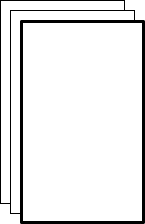
\includegraphics[scale=0.5]{stackview_wireframe}
	\centering
	\caption{Estrutura de um layout em pilha}
\end{figure}

No layout em pilha, o componente \textit{ToolBar.qml} será instanciado e posicionado no topo da janela do aplicativo. O \textit{ToolBar} verifica algumas propriedades da página ativa para permitir adicionar botões dinamicamente. É importante destacar que em ambos os layouts, somente uma página pode ser visualizada por vez.

\begin{figure}[H]
	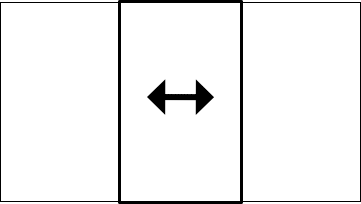
\includegraphics[scale=0.5]{swipeview_wireframe}
	\centering
	\caption{Estrutura de um layout em linha}
\end{figure}

No layout em linha, o componente \textit{TabBar.qml} será instanciado e posicionado no rodapé da janela do aplicativo e trabalhará em conjunto com o \textit{SwipeView}. A arquitetura suporta intercalar os dois layouts ao mesmo tempo, e um objeto \textit{Binding} do qml manterá o \textit{SwipeView} visível somente se não houver páginas na pilha do \textit{StackView}. No entanto, o \textit{SwipeView} será instanciado somente se a propriedade \textit{usesSwipeView} for definida para \textit{true} no arquivo de configuração.\par


\subsection{Requisitos funcionais suportados}
O projeto desta arquitetura visa atender quatro requisitos funcionais ententidos como básicos em todo sistema de informação, seja ele mobile ou não. Para atender aos requisitos, foi implementado APIs usando classes c++ nativas do Qt. Apesar de o qml dispôr de funcionalidades que poderiam atender aos quatro requisitos, foi decidido implementar em c++ por questões de desempenho devido menos código interpretado, melhor controle de consumo de memória e para simplificar a implementação de código nos plugins. Os requisitos listados a seguir, são disponibilizados pela arquitetura através de APIs de alto nível e podem ser utilizados por objetos qml. As APIs serão apresentadas em tópicos específicos posteriormente e os requisitos são:

\begin{enumerate}
	\item Acesso a rede para conexão com \textit{web services} via HTTP;
	\item Persistência de dados local via \textit{SQLITE};
	\item Notificações via \textit{push} e local;
	\item Comunicação entre objetos e plugins facilitado.
\end{enumerate}


\subsection{Visão Geral da Arquitetura}
A visão a seguir, apresenta um diagrama de pacotes e arquivos destacando uma visão lógica dos principais elementos da arquitetura. Logo a seguir, será descrito a responsabilidade e o conteúdo de cada um deles.

\begin{figure}[H]
	\includegraphics[scale=0.5]{diagrama_geral_da_arquitetura}
	\centering
	\caption{Pacotes principais da arquitetura}
\end{figure}

\begin{description}
	\item[1] \textit{tcc.pro}: Arquivo de configuração de todo projeto Qt. Nele é definido os módulos do Qt a serem utilizados na aplicação, as classes c++ que serão compiladas e linkadas no executável, os aquivos qrc que mapeiam os componentes qml, as imagens e arquivos genéricos a serem empacotados no aplicativo, além de módulos e arquivos de configuração para cada plataforma (linux, osx, android e ios). É neste arquivo que fica definido onde os plugins serão instalados no dispositivo.

	\item[2] \textit{main.cpp}: Arquivo que inicializa a aplicação. Esse arquivo é responsável por instanciar as classes do Qt que exibem a janela do aplicativo e o interpretador de código qml, além de classes da camada de aplicação, configuração e utilitários. O \textit{main.cpp} também é responsável por carregar os arquivos de tradução e registrar objetos no contexto da aplicação a serem utilizados pelos plugins.

	\item[3] \textit{config.json}: Arquivo de configuração principal desta arquitetura, pois contém propriedades que indicarão alguns comportamentos iniciais e escolha de tipos de objetos a serem instanciados, tais como, exibir os termos de uso na primeira inicialização do aplicativo (carregará o arquivo \textit{assets/eula.html} definido pelo desenvolvedor), se tem login ou não (caso sim, instanciará um objeto que gerencia o perfil do usuário e exibirá a página de login na inicialização), se usará layout em linha e etc. Os detalhes deste arquivo serão apresentados em um tópico mais adiante.

	\item[4] \textit{src}: Diretório de código fonte. É onde está as classes c++, componentes qml utilizados internamente e dispostos para os plugins como componentes reusáveis. Esse diretório é sub-dividido em outros cinco diretórios que organizam as classes c++ por tipo de API e são eles:

	\begin{itemize}
		\item \textit{core}: contém classes do núcleo da aplicação dentre elas \textit{App}, \textit{PluginManager}, \textit{Notification} e \textit{Utils};
		\item \textit{database}: contém classes da API de persistência de dados;
		\item \textit{extras}: contém classes de customização de estilo no android;
		\item \textit{network}: contém as classes da API de rede;
		\textit{qml}: contém os arquivos qml sub-divididos em \textit{private} e \textit{public}, sendo os componentes "privado" os que são utilizados internamente pela aplicação e os componentens públicos os que são reutilizados pelos plugins.
	\end{itemize}

	\item[5] \textit{plugins}: Diretório de plugins. Cada plugin deve obrigatóriamente estar em um sub-diretório com no mínimo um arquivo de configuração de nome \textit{config.json} e os arquivos qml necessários para o seu funcionamento. Os detalhes dos requisitos para o carregamento de um plugin serão descrito em um tópico posterior.

	\item[6] \textit{translations}: Diretório contendo os arquivos de tradução. Os arquivos de tradução devem ser gerados ou atualizados antes de cada release do aplicativo. Um arquivo de resources \textit{translations.qrc} existe neste diretório e deve ser utilizado para mapear os arquivos de idioma suportados pelo aplicativo. Cada arquivo de tradução deve ser nomeado seguindo o padrão \textit{language\_COUNTRY} com extensão \textit{ts}, por exemplo: \textit{pt\_BR.ts}. Ao iniciar a aplicação, no \textit{main.cpp}, tentará identificar o \textit{locale} que define o idioma utilizado no dispositivo e o arquivo correspondente será carregado para que os textos visíveis sejam traduzidos para o usuário. Para gerar as traduções, deve-se utilizar o comando \textit{lupdate *.pro} (na raíz do projeto) para criar ou atualizar o arquivo \textit{ts} principal.

	\item[7] \textit{android}: Diretório contendo os arquivos de configuração do aplicativo para a plataforma android. Outros sub-diretórios guardam arquivos do \textit{gradle} utilizados para o \textit{build} do APK, ícones do lançador do aplicativo e classes java, além de uma versão da lib \textit{openssl} compilada para o funcionamento de requisições HTTP.

	\item[8] \textit{assets}: Diretório contendo imagens e arquivos de configuração do \textit{qtquickcontrols2} além de um arquivo html que pode ser usado para exibir os termos de uso do aplicativo quando necessário (se a propriedade \textit{showEula} for definida para true no arquivo de configuração). Um arquivo de \textit{resources} \textit{assets.qrc} mapeia todos os arquivos contidos neste diretório.

	\item[9] \textit{ios}: Diretório contendo os arquivos de configuração do aplicativo para a plataforma iOS. Pode conter os ícones do aplicativo e imagens requeridas pela plataforma, tais como as imagens de \textit{splash-screen}, além do arquivo de configuração \textit{Info.plist} que define nome e versão do aplicativo e os recursos do sistema requerido para o funcionamento da aplicação no iOS.
\end{description}


\subsection{Arquitetura de plugins}
As funcionalidades de um aplicativo baseado nesta arquitetura devem ser implementadas através de plugins, atendendo aos requisitos levantados para o aplicativo a ser desenvolvido utilizando apenas qml. Os plugins são independentes entre sí e podem incluir arquivos qml, txt, html e imagens em seu diretório. Qualquer componente de um plugin pode reutilizar os componentes públicos usando a diretiva \textit{import "qrc:/publicComponentes/"}, ao todo quinze componentes foram disponibilizados. Os plugins estão desacoplados do núcleo da aplicação e serão conhecidos em tempo de execução. Ao adicionar um novo plugin no diretório \textit{plugins}, ele será carregado no próximo \textit{build} do projeto. Para que um plugin seja identificado pelo objeto gerenciador de plugins e carregado na aplicação, é necessário obedecer a três restrições: 1ª estar em um sub-diretório dentro de \textit{plugins}; 2ª conter um arquivo \textit{config.json} dentro deste sub-diretório e 3ª conter pelo menos um arquivo qml visual ou \textit{listener}. Os \textit{listeners} são componentes não visuais que observam eventos da aplicação. O arquivo \textit{config.json} de um plugin deve ser um objeto contendo as seguintes propriedades:

\begin{enumerate}
	\item \textit{name} (string): o nome do plugin. Deve ser preenchido para que o plugin seja identificado pelo gerenciador de plugins;

	\item \textit{description} (string): um texto que descreve o plugin. Deve ser definido, caso contrário o plugin não será carregado;

	\item \textit{listeners} (array): uma lista de strings que indentifica os arquivos do plugin (componentes qml não visuais) que serão instanciados como observadores de eventos. O preenchimento dessa propriedade é opcional e pode ser preenchida mesmo que a propriedade \textit{pages} seja preenchida;

	\item \textit{pages} (array): uma lista de objetos que indentifica as páginas do plugin que serão acessadas a partir dos menus do aplicativo e deve ser preenchido se a propriedade \textit{listeners} estiver vazia.
\end{enumerate}

Cada objeto em \textit{pages} poderá conter as seguintes propriedades:

\begin{itemize}
	\item \textit{qml} (string): O nome do arquivo correspondente a página. Se essa propriedade não for definida, a página não será carregada;

	\item \textit{title} (string): O título correspondente a página a ser exibido no menu. Esse valor também é requerido, se não for definido, a página não será adicionada ao menu;

	\item \textit{awesomeIcon} (string) (opcional): O nome de um ícone do \textit{Awesome Icons} que será exibido no menu, em conjunto com o título. Se esse valor não for definido, um ícone padrão (\textit{gear}) será utilizado;

	\item \textit{roles} (array): Uma lista de strings contendo os nomes de perfil de usuário que poderão acessar a página. Essa lista será útil somente se for definido o tipo de perfil do usuário no objeto \textit{userProfile}. O objeto \textit{userProfile} é \textit{null} por default e será instanciado na inicialização do aplicativo se a propriedade \textit{usesLogin} for definida para \textit{true} no arquivo de configuração. Caso \textit{roles} não for definido, será setado um array vazio. Porém, se \textit{userProfile} for instanciado e definido uma string com o perfil do usuário na propriedade \textit{profile} e essa string não tiver em \textit{roles}, a página não será exibida. Informações sobre o objeto \textit{userProfile} será detalhado em um tópico posterior;

	\item \textit{order} (int): Um valor numérico que define a ordem em que a página será exibida na lista de itens nos menus. O desenvolvedor deverá definir um valor acima de zero e quanto maior o valor, maior a prioridade na lista de itens;

	\item \textit{isLoginPage} (bool): Um valor boleano que indica se a página representa a tela de login do aplicativo e deve ser definido se o valor da propriedade \textit{usesLogin} for definido para true no arquivo de configuração do projeto. Se o aplicativo usa login, o \textit{path} da página definida como login será persistido pois será lido por funções internas do aplicativo na inicialização e quando o usuário fizer \textit{logout}. Se mais de uma página for definida como \textit{loginPage} entre os plugins, será utilizada a última página identificada pelo gerenciador de plugins;

	\item \textit{isHomePage} (bool): Um valor boleano que indica se a página corresponde a primeira página exibida para o usuário e deve ser utilizado pela página correspondente quando o layout em pilha estiver sendo utilizado. O \textit{path} dessa página será persistido durante o carregamento dos plugins e será carregada por funções internas na inicialização quando não houver (ou após) o login. Se mais de uma página for definida como \textit{homePage}, será utilizada a última página identificada pelo gerenciador de plugins;

	\item \textit{showInDrawer} (bool): Um valor boleano que indica se a página poderá ser exibida no menu de layout em pilha (\textit{drawer menu}). Por padrão, o menu de layout em pilha será carregado. Porém, poderá ser instanciado no layout em linha se a propriedade \textit{usesDrawer} for definida para \textit{true} no arquivo de configuração. O layout em linha utiliza uma barra de botões como menu e com isso, é possível permitir acesso a páginas diferentes a partir dos dois menus;

	\item \textit{showInTabBar} (bool): Um valor boleano que indica se a página poderá ser exibida no menu de layout em linha. O objetivo dessa propriedade é permitir exibir páginas diferentes nos menus quando o \textit{drawer menu} menu estiver sendo utilizado.
\end{itemize}

As páginas serão instanciadas sob demanda quando o aplicativo tiver utilizando o layout em pilha, neste caso quando o usuário clicar em um item da lista no menu, a página correspondente será instanciada e ficará visível para o usuário. No layout em pilha, o menu é exibido pelo componente \textit{Menu.qml} que consiste de uma instância do objeto \textit{Drawer} do \textit{QuickControls} e as páginas serão listadas verticalmente. A figura a seguir apresenta um exemplo deste menu com uma lista simples de páginas.

\begin{figure}[H]
	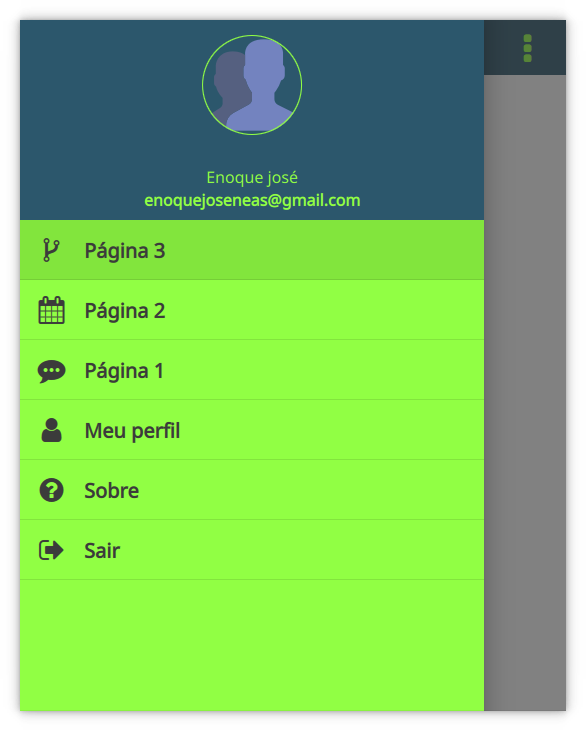
\includegraphics[scale=0.5]{exemplo_menu_layout_em_pilha}
	\centering
	\caption{Lista de páginas exibidas no menu de layout em pilha}
\end{figure}

Quando o layout em linha estiver sendo utilizado, uma lista horizontal de botões será acidionado no rodapé da janela do aplicativo permitindo ao usuário alternar entre as páginas disponíveis. Porém, no layout em linha, todas as páginas serão instanciadas no início da aplicação e terá um botão associado a cada página. No layout em linha, o menu corresponde ao componente \textit{TabBar.qml} também do \textit{QuickControls} com algumas modificações. A figura a seguir apresenta um exemplo deste menu com uma lista simples de páginas. A exibição do título da página pode ser ocultada setando a opção \textit{showTabButtonText} para false no arquivo de configuração do projeto.

\begin{figure}[H]
	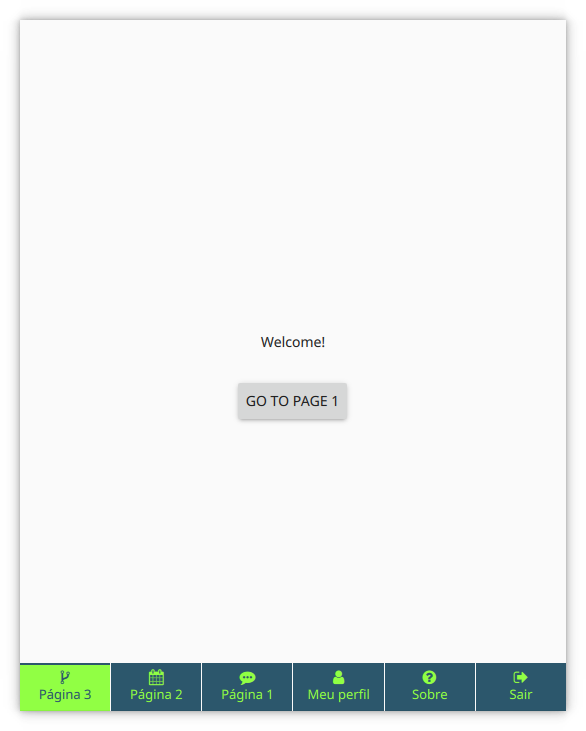
\includegraphics[scale=0.5]{exemplo_menu_layout_em_linha}
	\centering
	\caption{Lista de páginas exibidas no menu de layout em linha}
\end{figure}


\subsection{Gerenciamento de plugins}\label{sec:solucao-desenvolvida}
A classe \textit{PluginManager} é responsável por carregar os plugins, percorrendo todos os arquivos dentro do diretório \textit{plugins} e analizando as propriedades definida no arquivo \textit{config.json} de cada plugin. Em cada arquivo, é verificado as propriedades definida para cada página adicionando-a como objeto em um array. Após ler todos os plugins, o array de objetos é persistido nas configurações da aplicação para que na próxima inicialização não precise iterar novamente o diretório, lendo as definições dos plugins das configurações, exceto se houver uma atualização da aplicação ou quando a aplicação é executada em modo \textit{debug}. A cada inicialização, é feito uma verificação da versão do aplicativo, que também é persistida nas configurações, se houver diferença entre versão em execução da versão salva na execução anterior (se existir), os plugins serão recarregados. Além disso, esta classe também é reponsável por deletar todos os arquivos de cache contido no diretório de cache da aplicação a cada release. Outra responsabilidade dessa classe, é a criação da tabela de banco de dados do plugin se o plugin dispor de um arquivo \textit{plugin\_table.sql} em seu diretório. O banco de dados da aplicação é criado por um objeto que gerencia as operações de persistência e será detalhado em outro tópico. O diagrama a seguir, apresenta as operações e atributos da classe \textit{PluginManager}.

\begin{figure}[H]
	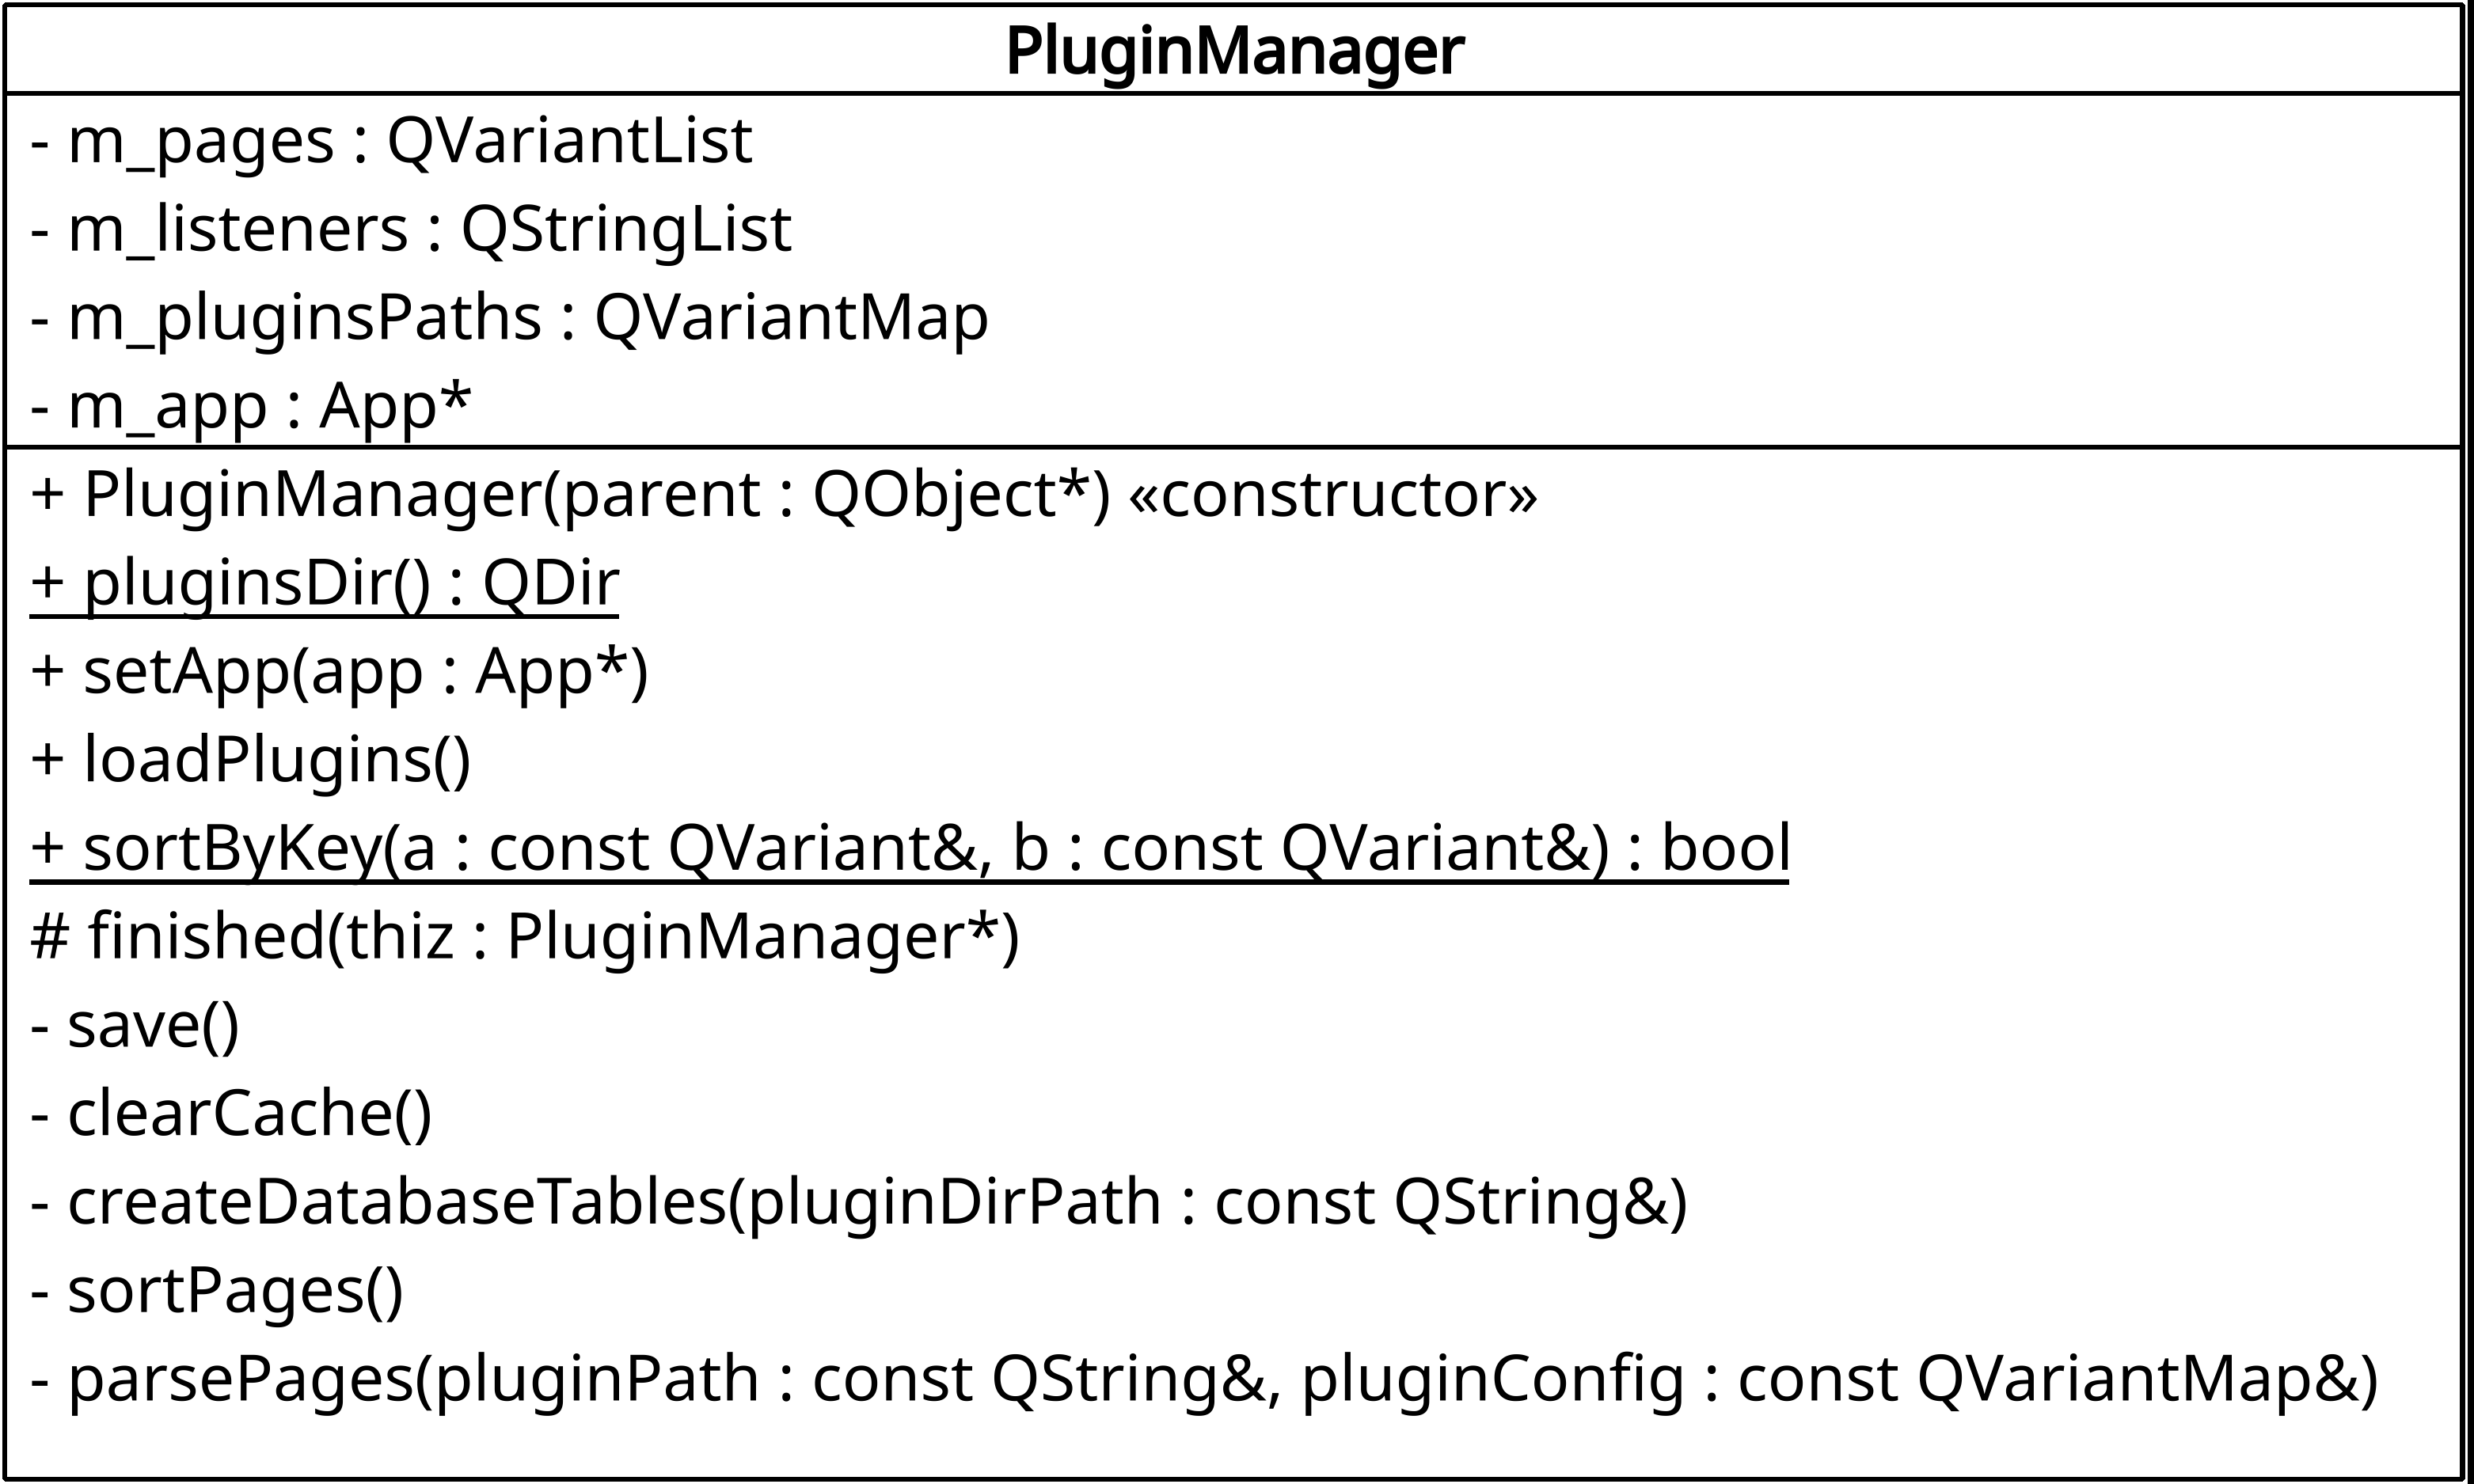
\includegraphics[width=8cm]{diagrama_de_classe_PluginManager}
	\centering
	\caption{Diagrama da classe PluginManager}
\end{figure}

O carregamento dos plugins é feito antes de instanciar qualquer componente visual, na invocação do método \textit{loadPlugins}. O objeto \textit{pluginManager} será destruido após o carregamento dos plugins para garantir baixo consumo de memória pelo aplicativo.


\subsection{A classe App}\label{sec:solucao-desenvolvida}
A classe \textit{App} é um componente importante nesta arquitetura, suas principais responsabilidades consiste de instanciar \textit{PluginManager}, carregar o arquivo \textit{config.json} que contém parâmetros da aplicação e gerenciar a persistência das configurações do aplicativo via \textit{QSettings}\footnote{https://doc.qt.io/qt-5/qsettings.html.}. \textit{App} também é responsável por notificar os objetos através do sinal \textit{eventNotify}. A classe \textit{App} é instanciada na inicialização do aplicativo e registrada no contexto da aplicação para que os plugins possam invocar seus métodos públicos. Por exemplo, o método \textit{readSettings} que retorna um tipo genérico de dado requerendo apenas um parâmetro que identifique o dado a ser retornado. Outra tarefa que corresponde a esta classe, é a criação de uma conexão com a atividade do aplicativo no android e no iOS. No android, essa atividade corresponde a um objeto java que delega eventos de toque na tela e acesso a recursos do dispositivo para os objetos do Qt. A aplicação poderá receber parâmetros de eventos como \textit{push notification} ou token de registro no \textit{Firebase}, quando o serviço de push for utilizado. O registro do token e o recebimento de notificações via push é feito por objetos nativos de cada plataforma em um processo separado da aplicação, e em tempo de execução as atividade passará o token ou os argumentos recebidos do push para o aplicativo através de uma chamada ao método estático \textit{fireEventNotify} da classe \textit{App} que irá dispará para objetos observadores definido pelo desenvolvedor. A figura abaixo apresenta o diagrama de classe da classe \textit{App}.

\begin{figure}[H]
	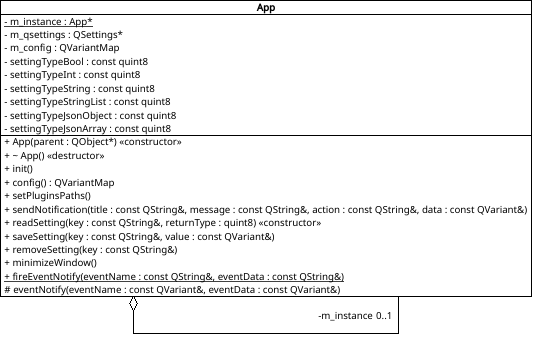
\includegraphics[scale=0.6]{diagrama_de_classe_App}
	\centering
	\caption{Diagrama da classe App}
\end{figure}

\textit{App} é quem define o estilo de \textit{widgets} utilizado pelos componentes qml. O tipo de estilo deve ser definido pelo desenvolvedor no arquivo de configuração na propriedade \textit{applicationStyle} e será passado diretamente para o objeto \textit{QQuickStyle}. Os possíveis valores para esta propriedade serão detalhados na sessão que descreve o arquivo \textit{config.json}. A instância da classe \textit{App} adicionará no objeto \textit{Config} uma propriedade contendo o path de cada plugin para facilitar o acesso aos arquivos no diretório de cada plugin. Por exemplo, considerando que \textit{Session} é um plugin, os arquivos em seu diretório poderão ser acessados da seguinte forma: \textit{Config.plugins.session + "File.qml"}.


\subsection{Gerenciamento de configurações}
A arquitetura provê uma API simples e de alto nível para persistir dados utilizando o conceito \textit{chave.valor} através do objeto \textit{App}. Nesse mecanismo, a chave identifica o dado a ser armazenado e o valor é o dado a ser persistido. Os tipos de dados válidos são: strings, números, objetos ou arrays e os métodos disponíveis podem ler, persistir ou apagar dados nas configurações do aplicativo. Os métodos serão descritos a seguir:
	\begin{itemize}
		\item \textit{readSetting}: Utilizado para ler um dado persistido utilizando uma string como parâmetro. O parâmetro deve identificar a informação a ser lida. Por padrão, o tipo de dado a ser retornado é string, porém, se o dado não for string o segundo parâmetro deve ser passado indicando o tipo específico a ser retornado. Os tipos possíveis são: \textit{SettingTypeBool} - para retornar um valor boleano; \textit{SettingTypeInt} - para retornar um inteiro; \textit{SettingTypeStringList} - para retornar uma lista de strings; \textit{SettingTypeJsonObject} - para retornar um objeto javascript; \textit{SettingTypeJsonArray} - para retornar um array de objetos javascript. Os tipos devem ser especificados para evitar o uso de cast no qml.

		\item \textit{saveSetting}: Utilizado para persistir dados. Esse método é \textit{void} e possui dois parâmetros que devem ser passados. O primeiro é uma string que identifica o valor a ser persistido, e o segundo é o dado propriamente dito. O dado pode ser uma string, um valor numérico, um objeto ou array.

		\item \textit{removeSetting}: Utilizado para apagar alguma informação persistida. Esse método requer como parâmetro uma string que indentifica o valor a ser deletado.
	\end{itemize}

O código a seguir, apresenta um exemplo de persistência e leitura de dados usando o mecanismo \textit{chave.valor}:

\begin{center}
\begin{lstlisting}[
	language=qml,
	basicstyle=\small,
	showspaces=false,
	showstringspaces=false,
	keywordstyle=\color{red}
]

import QtQuick 2.8

Item {
    Component.onCompleted: {
	var foo = App.readSetting("foo")
	if (bar != foo)
	   App.saveSetting("foo", bar)
    }
}
\end{lstlisting}
\captionof{lstlisting}{Exemplo de persistência através do objeto \textit{App}}
\end{center}


\subsection{Gerenciamento de eventos}
A classe \textit{App} possui o sinal \textit{eventNotify} e deve ser utilizado pelos plugins e objetos como conector. Este sinal possui dois parâmetros: o primeiro é uma string que identifica o evento e o segundo, um objeto que corresponde ao dado ou argumento emitido no evento. Como uma instância da classe \textit{App} é adicionada ao contexto da aplicação, objetos podem disparar eventos fazendo uma chamada ao sinal da seguinte forma: \textit{App.eventNotify(nome\_do\_evento, argumento)}. Observadores devem criar uma conexão com este sinal utilizando o objeto \textit{Connections} do qml, especificando como \textit{target} o objeto \textit{App}. A figura a seguir, apresenta um exemplo de código para uma conexão com este sinal:

\begin{center}
\begin{lstlisting}[
	language=qml,
	basicstyle=\small,
	showspaces=false,
	showstringspaces=false,
	keywordstyle=\color{red}
]
import QtQuick 2.8

Connections {
    target: App
    onEventNotify: {
        if (eventName == Config.events.someEvent)
            foo()
    }
}
\end{lstlisting}
\captionof{lstlisting}{Exemplo de conexão com o sinal \textit{eventNotify}}
\end{center}


\subsection{O Arquivo de Configuração}\label{sec:solucao-desenvolvida}
O arquivo \textit{config.json} é um componente importante desta arquitetura, ele é utilizado como arquivo de configuração geral do aplicativo, porém, suas informações não são persistidas. O conteúdo deste arquivo será repassado para a aplicação como um objeto javascript e o usuário poderá adicionar propriedades a serem lidas pelos plugins. No entanto, as propriedades fornecidas no modelo desta arquitetura não devem ser removidas, pois, componentes internos fazem uso das propriedades definidas neste arquivo. Os plugins poderão ler essa propriedade acessando \textit{Config.\_nome\_da\_propriedade}. As principais propriedades e seus possíveis valores podem ser entendidas a seguir:

\begin{itemize}
	\item \textit{appName} (string): O nome do aplicativo. Este valor será setado em \textit{QApplication.setApplicationName} na inicialização do aplicativo;

	\item \textit{appDescription} (string): Uma descrição sobre o aplicativo. Essa propriedade é opcional;

	\item \textit{organizationName} (string): O nome da organização. Este valor será setado em \textit{QApplication.setOrganizationName} na inicialização do aplicativo e é será utilizado internamente pelo Qt para definir o nome do diretório de configurações da aplicação;

	\item \textit{organizationDomain} (string): O domínio da organização, como por exemplo \textit{qt.project.org}. É utilizado pelo Qt internamente.

	\item \textit{applicationStyle} (string): O nome do estilo a ser aplicado nos widgets (\textit{Button}, \textit{TabBar}, \textit{ToolTip} e etc.). Os possíveis valores são: \textit{Material}, \textit{Universal} e \textit{Default}. O valor dessa propriedade será passada pelo objeto \textit{App} para \textit{QQuickStyle.setStyle};

	\item \textit{forceEulaAgreement} (bool): Um valor boleano que inidica se a aplicação deverá exigir do usuário confirmação de aceitação dos termos de uso para continuar usando o aplicativo. Esse valor só terá efeito se a propriedade \textit{showEula} for definida para \textit{true};

	\item \textit{hasLogin} (bool): Um valor boleano que indica se o aplicativo deverá carregar uma página de login na inicialização. Se definido para \textit{true}, a aplicação irá utilizar a página (dentre os plugins) que definiu \textit{isLoginPage} para \textit{true}, identificada pelo gerenciador de plugins durante o carregamento dos plugins;

	\item \textit{showEula} (bool): Um valor boleano que inidica se a aplicação exibirá para o usuário uma página contendo os termos de uso do aplicativo. Caso seja setado para \textit{true}, o arquivo \textit{assets/eula.html} será carregado e exibido na página incial, na inicialização do aplicativo. Após o usuário ler e acitar os termos de uso, o usuário irá para a página de login ou \textit{home page} se tiver sido definida;

	\item \textit{showTabButtonText} (bool): Um valor boleano que indica se o título da página será exibida no botão do menu em linha, que consite de um objeto \textit{TabButton} do \textit{QuickControls}. Essa propriedade só terá efeito quando a aplicação tiver usando o layout em linha.

	\item \textit{usesSwipeView} (bool): Um valor boleano que indica se o layout principal do aplicativo será em linha, que consiste na utilização de um container do \textit{QuickControls} \textit{SwipeView}. No entanto, o container responsável pelo layout em pilha, \textit{StackView} ainda continuará disponível na aplicação, porém como container secundário. Um objeto fará o \textit{Binding} entre ambos os containers, ocultando o \textit{SwipeView} quando alguma página for adicionada a pilha do \textit{StackView}. No \textit{SwipeView} o usuário poderá alternar entre as páginas deslizando horizontalmente.

	\item \textit{usesDrawer} (bool): Um valor boleano que indica se o menu lateral usado no layout em pilha, será instanciado. Esse componente corresponde a um objeto \textit{Drawer} do \textit{QuickControls}. No entando, esse flag terá efeito apenas no layout em linha, ou seja, se \textit{usesSwipeView} for true, pois no layout em pilha ele será instanciado mesmo que esse flag seja falso. O objetivo dessa propriedade é permitir que o programador possa utilizar o menu lateral quando o layout for me linha, intercalando as páginas que serão visíveis em cada um dos menus através das propriedades \textit{showInDrawer} e \textit{showInTabBar} na configuração de cada página no arquivo de configuração do plugin.

	\item \textit{showDrawerImage} (bool): Um valor boleano que indica se a imagem do \textit{Drawer} menu será carregada. Por padrão a imagem não será exibida.

	\item \textit{restService} (objeto): Um objeto contendo as definições do serviço REST, como url base e o tipo de autenticação seguido dos respectivos parâmetros a serem enviados nas requisições HTTP como token ou usuário e senha. As propriedades para \textit{restService} são: 

	\begin{itemize}
		\item \textit{basicAuthentication} (objeto): Um objeto que contém os parâmetros de autenticação básica a ser passara no cabeçalho das requisições HTTP, caso o \textit{webservice} exija authorização nas requisições. Esse objeto é formato por duas propriedades: o\textit{userName} e o \textit{userPass}. O \textit{basicAuthentication} é uma maneira simples de lidar com autenticação utilizando um parâmetro no cabeçalho HTTP, normalmente \textit{nome de usuário: senha} codificado em um hash \textit{base64}.

		\item \textit{baseUrl} (string): A url base do serviço REST. Essa propriedade será utilizada pelo objeto \textit{RequestHttp} nos métodos de requisição ao serviço REST GET, POST e etc. O objetivo é que nas páginas que fazem requisições HTTP adicionem apenas o \textit{path}, a fim de reduzir e simplificar o código. Com isso, uma alteração futura da url do serviço REST seria feita apenas no arquivo de configuração. Por exemplo, uma requisição do tipo GET pode ser feita da seguinte forma: \textit{requestHttp.get("/get-messages?page=2")}. Internamente, o objeto gerenciador de requisições concatenará essa propriedade com o path.

		\item \textit{baseImagesUrl} (string): A url base dos arquivos de imagens, caso o serviço REST utilize uma url diferente ou um sub-domínio para os resources.
	\end{itemize}

	\item \textit{fontSize} (objeto): Um objeto com as definições de valores inteiros para os tamanhos de fonte a serem utilizadas em elementos textuais como \textit{labels}. Essa propriedade possui 4 atributos: \textit{small}, \textit{normal}, \textit{large} e \textit{extraLarge};

	\item \textit{theme} (objeto): Um objeto com as definições de cores utilizada nos elementos visuais, tais como Botões, \textit{ToolBar}, \textit{TabBar}, cor de fundo das páginas e etc.;

	\item \textit{events}: (objeto): Um objeto que mapeia os identificadores de eventos, baseados em um par de strings \textit{nome-do-evento.valor}. Essa propriedade deverá ser utilizada por objetos e componentes internos para identificarem de qual evento estão sendo notificados, a fim de padronizar os nomes dos eventos e reduzir a replicação de strings na aplicação. O objeto \textit{App} adiciona treze nomes de eventos, alguns são utilizados somente por objetos internos, outros podem ser utilizados pelos plugins para executarem ações específicas em dado momento. Esses eventos serão descritos a seguir:

	\begin{itemize}
		\item \textit{cameraImageSaved} (string): Utilizado para notificar observadores que uma imagem foi capturada pela câmera do dispositivo e salva localmente. A url da imagem salva será passado no segundo argumento do evento;

		\item \textit{cancelSearch} (string): Utilizado pelo \textit{ToolBar} para indicar que o campo de busca não está ativo, para que a página corrente atualize o conteúdo para o usuário. O \textit{ToolBar} possui um campo texto para pesquisa e ficará visível quando a página alterar o valor da propriedade \textit{toolBarStatus} para \textit{"search"}. Essa funcionalidade permitirá que uma página filtre os resultados exibidos na sua \textit{view}, recebendo em um atributo string \textit{searchText} o valor digitado no campo. Esse recurso funcionará somente no layout em pilha. O usuário poderá cancelar a busca clicando em um botão voltar que ficará visível ao lado do campo de busca, nesse momento, o sinal \textit{"cancelSearch"} será disparado;

		\item \textit{logoutApplication} (string): Utilizado pelo objeto \textit{UserProfile} para atualizar o status da propriedade \textit{isUserLoggedIn} para false e em seguida, focar na página de login. Esse evento deve ser utilizado para evitar o acesso direto ao objeto \textit{UserProfile} pelos plugins, e deve ser emitido sempre que desejar remover todas as páginas da pilha (caso o layout seja em pilha) ou desabilitar o acesso as páginas do aplicativo (no layout em linha);

		\item \textit{newIntentPushMessage} (string): Esse evento é utilizado pelas APIs de notificação do android e iOS quando o usuário clicar em uma notificação na bandeija do sistema contendo algum dado na notificação. O segundo parâmetro do sinal \textit{eventData} conterá os dados da mensagem em uma string e caso seja um json, é necessário fazer o parse;

		\item \textit{newPushMessage} (string): Esse evento será disparado sempre que uma notificação via push chegar no dispositivo e o mesmo estiver em execução em \textit{foreground} ou \textit{background}. Ele é disparado a partir dos serviços de notificação que executam em outro processo e serão passados para a aplicação através de uma conexão entre o objeto java \textit{QtAtivity} no android e o \textit{QtAppDelegate} no iOS. O segundo parâmetro do sinal \textit{eventData}, conterá os dados da mensagem em uma string e caso seja um objeto json, é necessário fazer o parse;

		\item \textit{newPushNotificationToken} (string): Esse evento será emitido quando o token de registro no serviço do Firebase for realizado. Esse evento será disparado pelos objetos do \textit{Firebase}, que executam em outro processo e serão passados para a aplicação através de uma conexão entre o objeto java \textit{QtAtivity} no android e o \textit{QtAppDelegate} no iOS. O segundo parâmetro do sinal \textit{eventData} conterá os dados da mensagem em uma string e caso seja um objeto json, é necessário fazer o parse;

		\item \textit{openDrawer} (string): Esse sinal deve ser disparado para que o \textit{Drawer Menu} seja aberto, evitando uma chamada direta ao objeto. O \textit{ToolBar} por exemplo, emite esse sinal quando o usuário clicar no ícone do menu;

		\item \textit{popCurrentPage} (string): Esse evento deve ser disparado sempre que uma página precise ser removida da pilha do \textit{StackView} (container do layout em pilha). Inicialmente esse sinal é disparado pelo \textit{ToolBar} e ouvido pelo \textit{PageStack}.

		\item \textit{refreshDrawerPages} (string): Esse evento pode ser utilizado para atualizar a lista de itens no \textit{Drawer} menu permitindo adicionar páginas dinamicamente.

		\item \textit{requestUpdateUserProfile} (string): Esse evento deve ser emitido quando houver um perfil de usuário no aplicativo e permitirá atualizar as informações ou dados do usuário no objeto \textit{UserProfile.profile}. Por exemplo, uma página que permite editar os dados do usuário em um formulário, ao clicar em atualizar alguma informação, a página poderá emitir esse evento passando como argumento um objeto contendo as informações do usuário no estilo \textit{chave.valor}.

		\item \textit{initUserProfile} (string): Esse evento também deve ser emitido quando houver um perfil de usuário no aplicativo, e um objeto contendo os dados do usuário deverá ser enviado como argumento do sinal, contendo no mínimo as propriedades "id" e "email". Um exemplo de uso deste sinal, pode ser emitido pela página de login, após sucesso na autenticação, requisitando que a página definida como \textit{home page} seja instanciada e os dados do usuário sejam inicializados.

		\item \textit{setUserProfileData} (string): Esse é outro evento para uso com o perfil de usuário no aplicativo, e visa adicionar ou atualizar uma única informação no perfil do usuário. Logo, o argumento do sinal deve conter a propriedade \textit{key} contendo o nome da propriedade a ser adicionada e \textit{value} contendo o seu respectivo valor. Por exemplo, o seguinte objeto pode ser utilizado como argumento deste sinal: \textit{\{"key": "username", "value": "enoque"\}}.

		\item \textit{userProfileChanged} (string): Esse evento será emitido pelo objeto \textit{UserProfile} sempre que ocorrer alguma atualização nos dados do usuário. No parâmetro do sinal será passado uma referência para o objeto \textit{profile}.
	\end{itemize}
\end{itemize}


\subsection{Acesso a Rede (HTTP)}\label{sec:solucao-desenvolvida}
Um dos requisitos funcionais providos nesta arquitetura é o acesso a rede para comunicação com algum \textit{web service} via HTTP. O desenvolvedor deverá adicionar na propriedade \textit{restService.baseUrl} no arquivo de configuração, o endereço base do serviço rest e utilizar apenas o path da url nos objetos que realizam as requisições GET, POST e etc. Para realizar requisições HTTP, os plugins terão a disposição um objeto \textit{requestHttp} em cada página. Os objetos \textit{listeners} que precisarem fazer requisição HTTP podem utilizar o componente \textit{RequestHttp.qml} disponível na arquitetura. No entanto, se por algum motivo for preciso iniciar uma requisição para outro domínio diferente do serviço rest, basta passar a url completa no primeiro parâmetro dos métodos de requisição.\par

Para realizar requisições HTTP, foi criado uma classe c++ que encapsula requisição, autenticação, download e upload com o objetivo de oferecer um componente rico em recursos e de alto nível para os plugins. Essa classe utiliza componentes do Qt e não é utilizada diretamente pelos plugins, foi criado um arquivo qml com o mesmo nome da classe e disponibilizado como componente reutilizável na arquitetura. As subsessões a seguir descrevem os componentes correspondentes a API de rede provido nesta arquitetura.


\subsubsection{A classe RequestHttp}\label{sec:solucao-desenvolvida}
A classe \textit{RequestHttp} utiliza componentes do Qt para realizar as operações de rede, dentre elas \textit{QNetworkAccessManager} e \textit{QNetworkRequest} são as mais importantes. Essa classe disponibiliza quatro métodos públicos principais que serão descritos a seguir:

\begin{itemize}
	\item \textit{get}: realiza uma requisição HTTP do tipo GET exigindo apenas a url de destino. Esse método possui dois parâmetros opcionais, o primeiro deles é um objeto do tipo \textit{chave-valor} e se passado adicionará a url uma \textit{query-string}. O segundo parâmetro opcional é também um objeto e pode ser passado quando for necessário adicionar dados no cabeçalho da requisição. O sinal \textit{finished} será emitido quando a requisição finalizar passando dois argumentos: \textit{statusCode} um inteiro contendo o status da responsa (200, 400, 500) e um objeto \textit{response} contendo o dado da resposta enviado pelo servidor. Se o servidor responder um objeto json, a resposta será um \textit{QVariantMap} e se for um array json, o argumento será \textit{QVariantList}, caso contrário uma string.

	\item \textit{post}: realiza uma requisição HTTP do tipo POST exigindo a url de destino e o dado a ser enviado como post em formato string ou array de bytes. O terceiro parâmetro desse método é opcional e pode ser passando quando for necessário adicionar dados no cabeçalho da requisição. A resposta da requisição será também emitida no sinal \textit{finished} como foi descrito no item anterior.

	\item \textit{uploadFile}: realiza uma requisição HTTP do tipo POST ou PUT exigindo a url de destino e um array de \textit{path} de arquivos locais a serem enviados para o servidor. A requisição será do tipo \textit{multipart-formdata} e o terceiro parâmetro pode ser passado para adicionar dados no cabeçalho da requisição. Esse método emitirá o sinal \textit{uploadFinished} quando o \textit{upload} do arquivo for finalizado. Para cada arquivo enviado, será emitido o sinal \textit{uploadProgressChanged} contendo os bytes do arquivo e total enviado.

	\item \textit{downloadFile}: realiza uma requisição HTTP do tipo GET exigindo apenas uma lista de urls de arquivos a serem baixados para o dispositivo. Por padrão, os arquivos serão salvos no diretório público de \textit{downloads}. No entanto, o segundo parâmetro \textit{saveInAppDirectory} do tipo boleano (default false) pode ser utilizado para alterar o diretório de destino dos arquivos para uma pasta interna do aplicativo. Para cada arquivo salvo, o sinal \textit{downloadedFileSaved} será emitido passando o path do arquivo salvo localmente. Outro sinal \textit{downloadProgressChanged} será emitido passando dois argumentos, o primeiro indica o tamanho em bytes do arquivo que está sendo baixado e o segundo um valor inteiro indicando os bytes já baixados.
\end{itemize}

Os métodos descritos anteriormente são todos \textit{void} e assíncronos e são declarados como \textit{Q\_INVOKABLE}\footnote{htps://doc.qt.io/qt-5/qtqml-cppintegration-exposecppattributes.html} para permitir a criação de objetos desta classe por componentes qml dos plugins. Para pegar a resposta de uma requisição HTTP, é preciso criar uma conexão com o \textit{finished}. Esse sinal será emitido se não houver erros no pedido e logo após a resposta do servidor ser enviada. O sinal \textit{finished} passará dois argumentos, \textit{statusCode} inteiro indicado o status da resposta (200, 400, 500 e etc.) e \textit{response} contendo o dado enviado. Se o dado enviado for um json válido será enviado como objeto json, caso contrário, uma string contendo o dado bruto enviado pelo servidor\par

A propriedade \textit{status} (integer) declarada como \textit{Q\_PROPERTY} pode ser utilizada para \textit{bindings} com outros objetos qml e indicará o \textit{status} atual de uma requisição. Os possíveis valores para \textit{status} podem ser comparado com as seguintes meta-propriedades (útil para \textit{bindings}):

\begin{itemize}
	\item \textit{Error}: inidica um erro no pedido, quando o servidor não responder ou o status da requisição for zero;
	\item \textit{Finished}: indica que a requisição terminou e é setada em \textit{status} antes da emissão do sinal \textit{finished};
	\item \textit{Loading}: indica que a requisição está em andamento ou carregando;
	\item \textit{Ready}: indica que a requisição está pronta, é definida em \textit{status} no construtor do objeto \textit{RequestHttp} indicando que está pronto para inicar requisições e também, é setado após a emissão do sinal \textit{finished}.
\end{itemize}

O diagrama a seguir, apresenta os atributos e métodos da classe \textit{RequestHttp}:

\begin{figure}[h]
	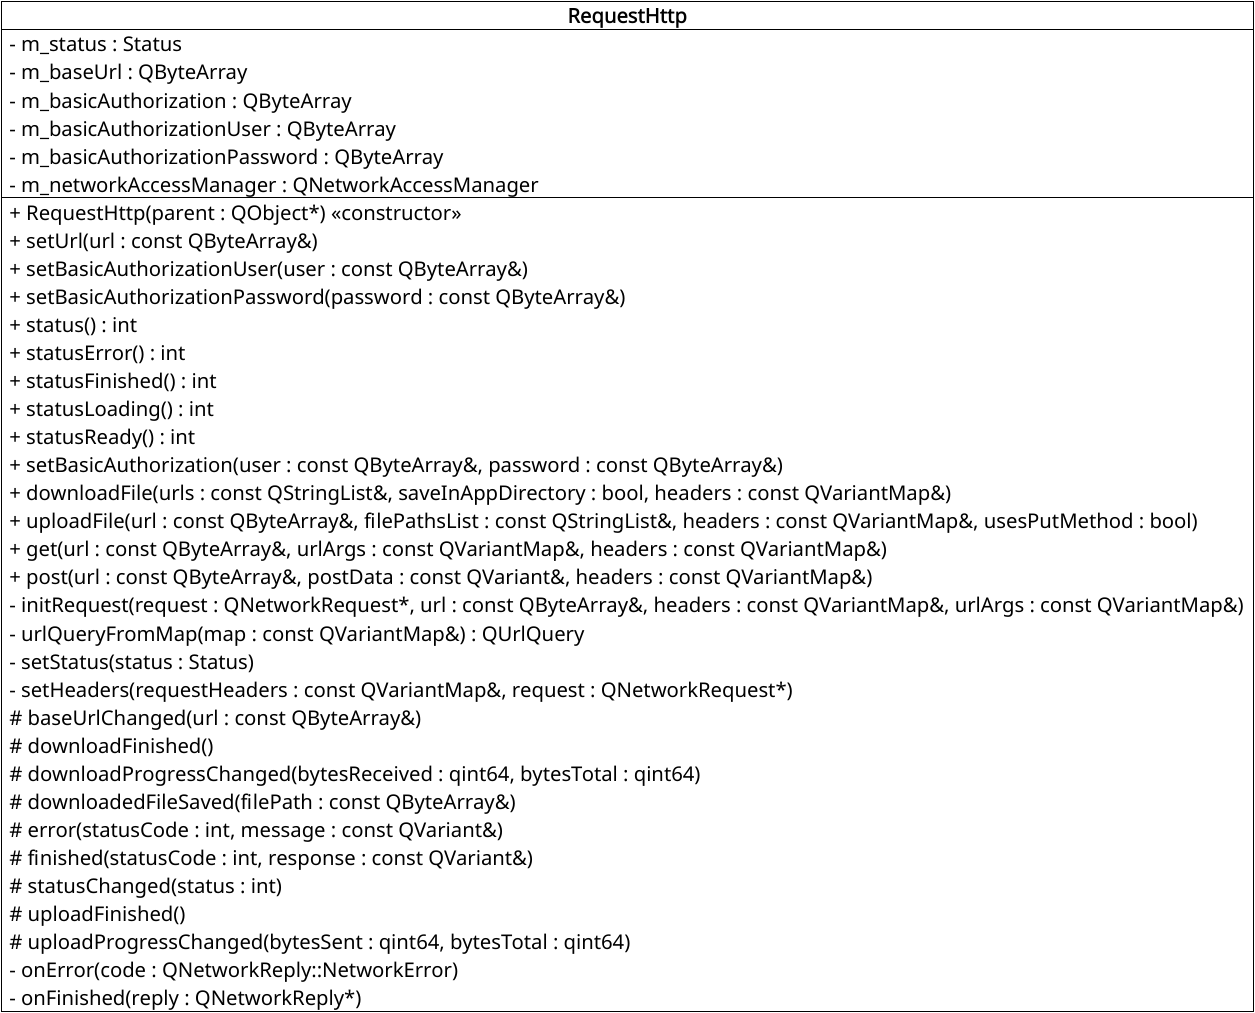
\includegraphics[width=8cm]{diagrama_de_classe_RequestHttp}
	\centering
	\caption{Diagrama da classe RequestHttp}
\end{figure}


\subsubsection{O Componente RequestHttp}\label{sec:solucao-desenvolvida}
A classe \textit{RequestHttp} é registrada como um tipo qml no contexto da aplicação e os plugins podem utilizá-la através da diretiva \textit{import RequestHttp 1.0} e declarando um objeto qml para utilizar seus métodos. No entando, para passar autenticação básica nas requisições é preciso setar os parâmetros do arquivo de configuração, além da url base. Logo, para simplificar o uso de requisições HTTP para os plugins, foi criado um arquivo qml \textit{RequestHttp.qml} que instancia a classe \textit{RequestHttp} e inicializa os artributos \textit{baseUrl}, \textit{basicAuthorizationUser} e \textit{basicAuthorizationPassword}, além de exibir mensagens de erros das requisições personalizadas para o usuário. O código a seguir, apresenta esse componente qml:

\begin{center}
\begin{lstlisting}[
	language=qml,
	basicstyle=\tiny,
	showspaces=false,
	showstringspaces=false,
	keywordstyle=\color{red}
]
import RequestHttp 1.0 

RequestHttp {
    baseUrl: Config.restService.baseUrl
    basicAuthorizationUser: Config.restService.basicAuthentication.userName
    basicAuthorizationPassword: Config.restService.basicAuthentication.userPass
    onError: {
	// trata e exibe mensagens de erro da requisicao
    }
}
\end{lstlisting}
\captionof{lstlisting}{Código do componente \textit{RequestHttp.qml}}
\end{center}


\subsection{Persistência de Dados}\label{sec:solucao-desenvolvida}
Persistência de dados é um requisitivo funcional disponibilizado nesta arquitetura e foi elaborada com o objetivo de fornecer aos plugins a possibilidade de persistir dados em um banco SQLITE. Cada plugin pode criar uma ou mais tabelas no banco de dados da aplicação e realizar as operações de inserção, atualização e busca de dados em suas tabelas, basta importar o componente Database com a diretiva \textit{import Database 1.0} e utilizá-lo para objeto qml. Para criar as tabelas no banco de dados da aplicação, o plugin deve fornecer um arquivo \textit{plugin\_table.sql} contendo os comandos de criação, alteração ou remoção das tabelas. Esse arquivo é lido pelo objeto gerenciador de plugins que passará o caminho do arquivo para outro objwto que criará a tabela. Esse arquivo será carregado e executado a cada release.\par

Para gerenciar as operações no banco de dados, foi criado uma classe c++ chamda de \textit{Database} que encapsula em métodos de alto nível as operações necessárias para criar o banco de dados, conectar e executar as \textit{querys sql}. No entanto, essa classe não é utilziada pelos plugins diretamente, foi criado uma outra classe chamada \textit{DatabaseComponent} que agrega uma instância de \textit{Database} e delega as operações para esse objeto. Através dessa API de persistência, os plugins poderão persistir e carregar dados com o dispositivo online ou até mesmo offline. Os tópicos a seguir apresenta detalhes de ambas as classes \textit{Database} e \textit{DatabaseComponent}.


\subsubsection{A classe Database}\label{sec:solucao-desenvolvida}
A classe \textit{Database} é responsável por criar o banco de dados \textit{SQLITE} na primeira execução do aplicativo se houver necessidade, ou seja, algum plugin dispor de um arquivo de criação de tabela \textit{plugin\_table.sql} em seu diretório. Se nenhum plugin fornecer esse arquivo, o banco de dados \textit{SQLITE} não será criado. A classe \textit{Database} utiliza as classes \textit{QSqlDatabase} e \textit{QSqlQuery} para criação e conexão com o banco de dados e a classe \textit{QSqlRecord} para as realizar \textit{querys}. Os métodos principais desta classe são descritos a seguir:

\begin{itemize}
	\item \textit{select}: Esse pode ser utilizado para recuperar dados de uma tabela através de uma consulta \textit{sql} e possui três parâmetros, o primeiro é nome da tabela onde será feito a consulta, o segundo é um objeto contendo os parâmetros da consulta (condição where) no estilo  \textit{nome-da-coluna.valor}, e o último parâmetro, um outro objeto contendo argumentos adicionais, tais como \textit{limit}, \textit{offset} e \textit{order by}. Esse método retornará uma lista de objetos resultante da consulta, se houver. Caso contrário, será retornado uma lista vazia;

	\item \textit{insert}: Esse método pode ser utilizado para inserir dados em uma tabela e os parâmetros requeridos são: o nome da tabela onde será feito a inserção e um objeto no estilo \textit{nome-da-coluna.valor} contendo os dados a serem persistidos. Se a inserção for efetuada com sucesso e a tabela possuir a coluna auto-incrementada como chave-primária o valor incrementado será retornado. Caso contrário, não possuir a coluna auto-incrementada, retornará o valor inteiro "1" (um) ou zero se houver erros na inserção;

	\item \textit{remove}: Esse método pode ser utilizado para deletar um ou mais registros em uma tabela específica. Esse método possui três parâmetros, o primeiro é o nome da tabela onde será feito a remoção, o segundo é um objeto contendo os argumentos ou filtros da \textit{query} no estilo \textit{nome-da-coluna.valor}. O terceito parâmetro é opcional e pode ser passado para customizar o operador de comparação para cada par no segundo parâmetro, por default é o operador de igualdade ("=");

	\item \textit{update}: Esse método pode ser utilizado para atualizar um registro em uma tabela específica. Os parâmetros desse método são basicamente os mesmos do método \textit{remove} descrito no item anterior, com uma adição, um parâmetro \textit{updateData} que consiste de um objeto contendo os dados a serem atualizados no estilo \textit{nome-da-coluna.valor}.
\end{itemize}

 O diagrama a seguir apresenta os atributos e métodos da classe \textit{Database}.
\begin{figure}[h]
	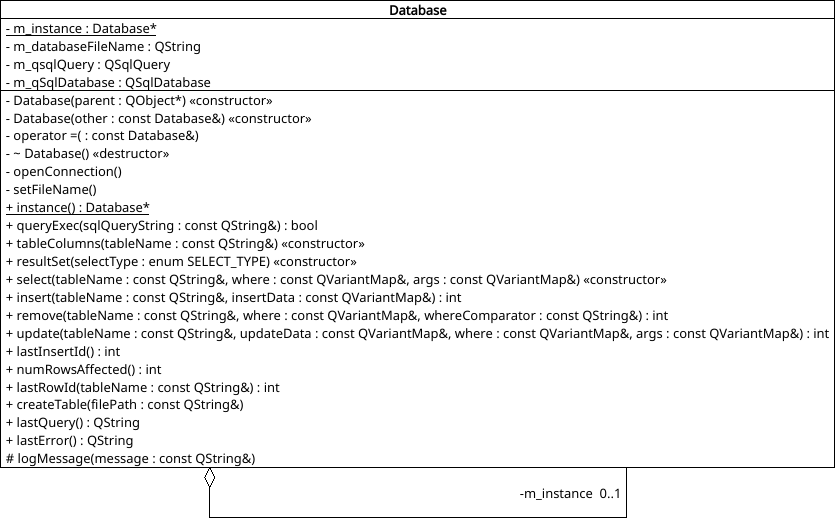
\includegraphics[width=8cm]{diagrama_de_classe_Database4}
	\centering
	\caption{Diagrama da classe Database}
\end{figure}


\subsubsection{A classe DatabaseComponent}\label{sec:solucao-desenvolvida}
A classe \textit{DatabaseComponent} foi criada com o objetivo de fornecer um componente rico em recursos e de alto nível para os plugins. Essa classe é registrada no contexto da aplicação como um tipo qml e permite aos plugins instanciarem como componentes qml. \textit{DatabaseComponent} agrega uma instância da classe \textit{Database} e delega as operações para esse objeto. No entanto, ela possui alguns atributos declarados como \textit{Q\_PROPERTY} que permitem aos plugins informar o nome da tabela no banco de dados, uma coluna chave-primária do tipo string, caso a tabela não utilize a coluna numérica id auto-incrementada, além de colunas que guardam objetos json para seja feito o parse quando algum registro for retornado para a view, a fim de evitar que a view faça parse utilizando javascript. Outro atributo \textit{totalItens} mantém atualizado o número de registros na tabela para fins de comparação eficiente com o número de itens disponível no serviço rest, útil para paginação de dados na view. O diagrama a seguir, apresenta os atributos e métodos dessa classe:

\begin{figure}[H]
	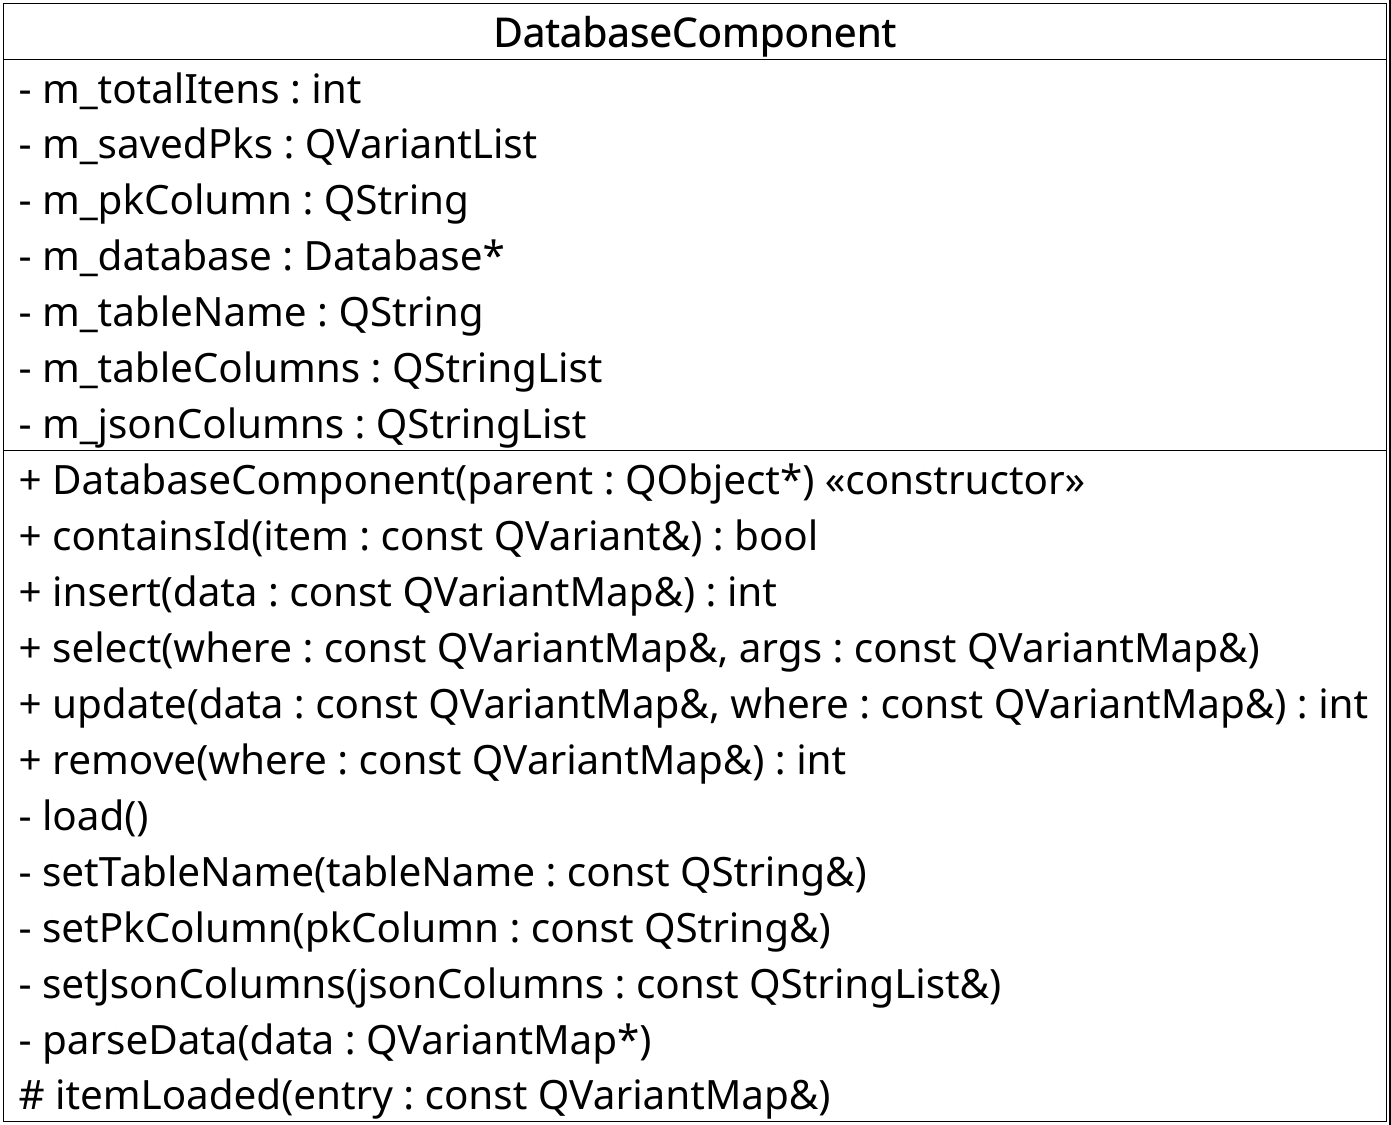
\includegraphics[width=8cm]{diagrama_de_classe_DatabaseComponent}
	\centering
	\caption{Diagrama da classe DatabaseComponent}
\end{figure}

É importante observar que os métodos de busca, inserção, remoção e atualização foram simplificados para que os objetos que utilizarem \textit{DatabaseComponent} informem apenas os parâmetros do método sem o nome da tabela. Outro recurso importante desse componente é que o método de busca é assíncrono e os resultados de uma busca, quando houver, será emitido no sinal \textit{itemLoaded} que passará como argumento um objeto contendo o nome da coluna e o dado armazenado. Essa classe possui ainda um método \textit{containsId} que verifica se um item (pela chave primária) já está salvo localmente a fim de sincronizar com a view os itens já baixados do serviço rest.

\subsection{Notificações do Sistema}
....


\subsection{Comunicação entre os objetos e plugins}
% Esta seção descreverá o processo de comunicação entre objetos no aplicativo e o uso correto dos eventos...
....


\subsection{O Componente UserProfile}\label{sec:solucao-desenvolvida}
....


\subsection{O Componente BasePage}\label{sec:solucao-desenvolvida}
....


\subsection{Componentes Visuais}\label{sec:solucao-desenvolvida}
....


\subsection{Fluxo de execução}\label{sec:solucao-desenvolvida}
....
%Adicionar um diagrama de sequência que mostre a inicialização, carregamento dos plugins e configuração geral do aplicativo%


\subsection{Métodos para utilização da arquitetura}
% descrever o README do projeto no github
Para se utilizar a arquitetura desenvolvida, deve-se seguir uma determinada ordem de atividades que serão descritos a seguir.
